\subsection{Artificial neural networks. Training.}


\acrlong{nn} are algorithms used in the field of \acrshort{ai} and try to solve problems in which one works with a large amount of data trying to find patterns in them. Furthermore, it is one of the few alternatives to other algorithms that are capable of treating large volumes of data.
\newline

The beginnings of neural networks date back to the 1950s, when McCulloch and WalterPitts \cite{kleene} worked on a mathematical model that resembled the behaviour of a neuron that they knew. The scientist Frank Rosenblatt, inspired by this work, developed what are known as networks of perceptions. This was the first approach to what is now known as neural networks \cite{nielsen}.


\subsubsection{Entrenamiento de una red}\label{training}
Como resumen de visto hasta ahora, para crear una red es necesario tener cuatro elementos distintos:
\begin{itemize}
\item Valores de entrada: Información con la que se va a predecir un dato o un conjunto de datos.
\item Estructura de la red: Esta es una información que se debe de conocer a priori antes de crear el modelo. Tiene distintas propiedades:
\begin{itemize}
    \item Número de capas: A mayor número de capas, mayor será el tiempo que tardará el modelo en computar el vector de salida $y$ porque mayor cantidad de cálculos tendrá que realizar. El número de capas junto con el número de neuronas por capa son parámetros importantes, puesto que un número muy bajo en el modelo y este no tendrá una buena precisión. Por lo contrario un número muy alto puede producir lo que se conoce como \textit{overfitting}(ver sección \ref{overfitting}).
    \item Número de neuronas en cada capa: Cabe destacar que el número de neuronas en la última capa será el tamaño del vector $y$, es decir, el número de etiquetas que el modelo predecirá.
    \item Función de activación por cada capa.
    \item Arquitectura de la red. % Se puede ver más información sobre los tipos de arquitecturas de redes en la sección TODO.
\end{itemize}
\item Las matrices $W$: Son matrices que recogen la información asociada a cada capa sobre los pesos $w$ y \textit{bias} $b$ de cada neurona de la red.
\end{itemize}

Las matrices $W$ son matrices con valores creados aleatoriamente. El proceso de entrenamiento de la red tratará de optimizar estas matrices para que el vector $y$ resultante sea lo más preciso posible. Para poder entrenar un modelo es necesario tener previamente un \textit{dataset} con un conjunto de vectores $x$ y su valor real. La cantidad de datos que proporcionemos al modelo para que aprenda está relacionada con la precisión del modelo. Con el ejemplo descrito en la Tabla \ref{tab:houses} se podrían usar las columnas \textit{tipo}, \textit{coords}, \textit{gc}, \textit{m2} y \textit{h} para predecir el valor $precio$.
\newline

Básicamente la red inicializa la matriz $W$ de forma aleatoria. El modelo dado un vector $x$ realiza todos los cálculos de cada neurona y devuelve un valor $y$ (o varios valores si la última capa tiene más de una neurona). $y$ es lo que el modelo ha predicho. Este proceso es el que se conoce como \textit{feed-forward}.
\newline

Para que la red aprenda, necesita primero saber si se ha equivocado y la magnitud del error. Si la magnitud de este error es muy grande, se deberá ajustar los valores de $W$ para minimizar el error. Por lo contrario, si el error es pequeño, no se ajustarán mucho los valores de $W$ porque realizando un ajuste en $W$ puede provocar una ligera mejoría en dicha predicción, pero puede desajustar otras predicciones que el modelo ha hecho previamente y eran también bastantes precisas. La elegancia de este algoritmo es que encuentra un balance entre lo que es ajustar valores para que la red aprenda y al mismo tiempo no desajustar demasiado para que la red se descompense en su aprendizaje global. Es la aplicación de la imitación del aprendizaje humano, un error con una gran repercusión deberá modificar comportamientos futuros, un error sin repercusión podrá ser ignorado o incorporar cambios proporcionados a las repercusiones.
\newline

El error se cuantifica con una función llamada función de coste o función de pérdida explicada en la sección \ref{costfunction}. A partir del valor del error, se usará un algoritmo que tratará de calcular la responsabilidad de cada neurona en dicho error y de esta forma poder ajustar los pesos y la \textit{bias} asociadas a dicha neurona. Este algoritmo se llama \textit{backpropagation} y es explicado en la sección \ref{backpropagation}.
\newline

Se puede pensar que este proceso se puede repetir infinitamente hasta tener un modelo perfecto, pero como se ve en la sección de \ref{overfitting} esto puede provocar que la red memorice el dataset que es usado para entrenar y no tenga la capacidad de generalizar. Por lo tanto, no solo se trata de ejecutar el algoritmo, sino que hay que realizar ciertas optimizaciones y tener varios conceptos en cuenta como por ejemplo: la selección de función de activación, diseño del vector de entrada y salida, métricas a usar, entre otros.
\newline

\label{p:company_backpropagation}
Como analogía para entender el algoritmo de \textit{backpropragation}, se puede usar la jerarquía de una empresa. Dicha empresa tras un trimestre desastroso elabora un resumen con los resultados. Estos resultados son equivalentes al error que el modelo produce. El jefe (la última capa de la red), tratará de rendir cuentas con los directivos. Estos directivos a su vez tratarán con otros directivos con menor responsabilidad y estos a su vez lo harán con jefes que estén por debajo suya y así sucesivamente hasta llegar al último nivel en la empresa (propagando el error hacia las capas más básicas). Posteriormente, la empresa elaborará un informe estudiando la responsabilidad de cada persona en el resultado del trimestre (que en el algoritmo de \textit{backpropagation} es conocido como el vector gradiente). Ese informe llegará al departamento de recursos humanos y este, tratará de modificar el comportamiento de cada trabajador en la empresa en función de su responsabilidad en el error (algoritmo del descenso del gradiente).
\newline

En el siguiente diagrama se puede visualizar el proceso que se lleva a cabo para entrenar una red neuronal: 
\begin{figure}[H]
    \centering
    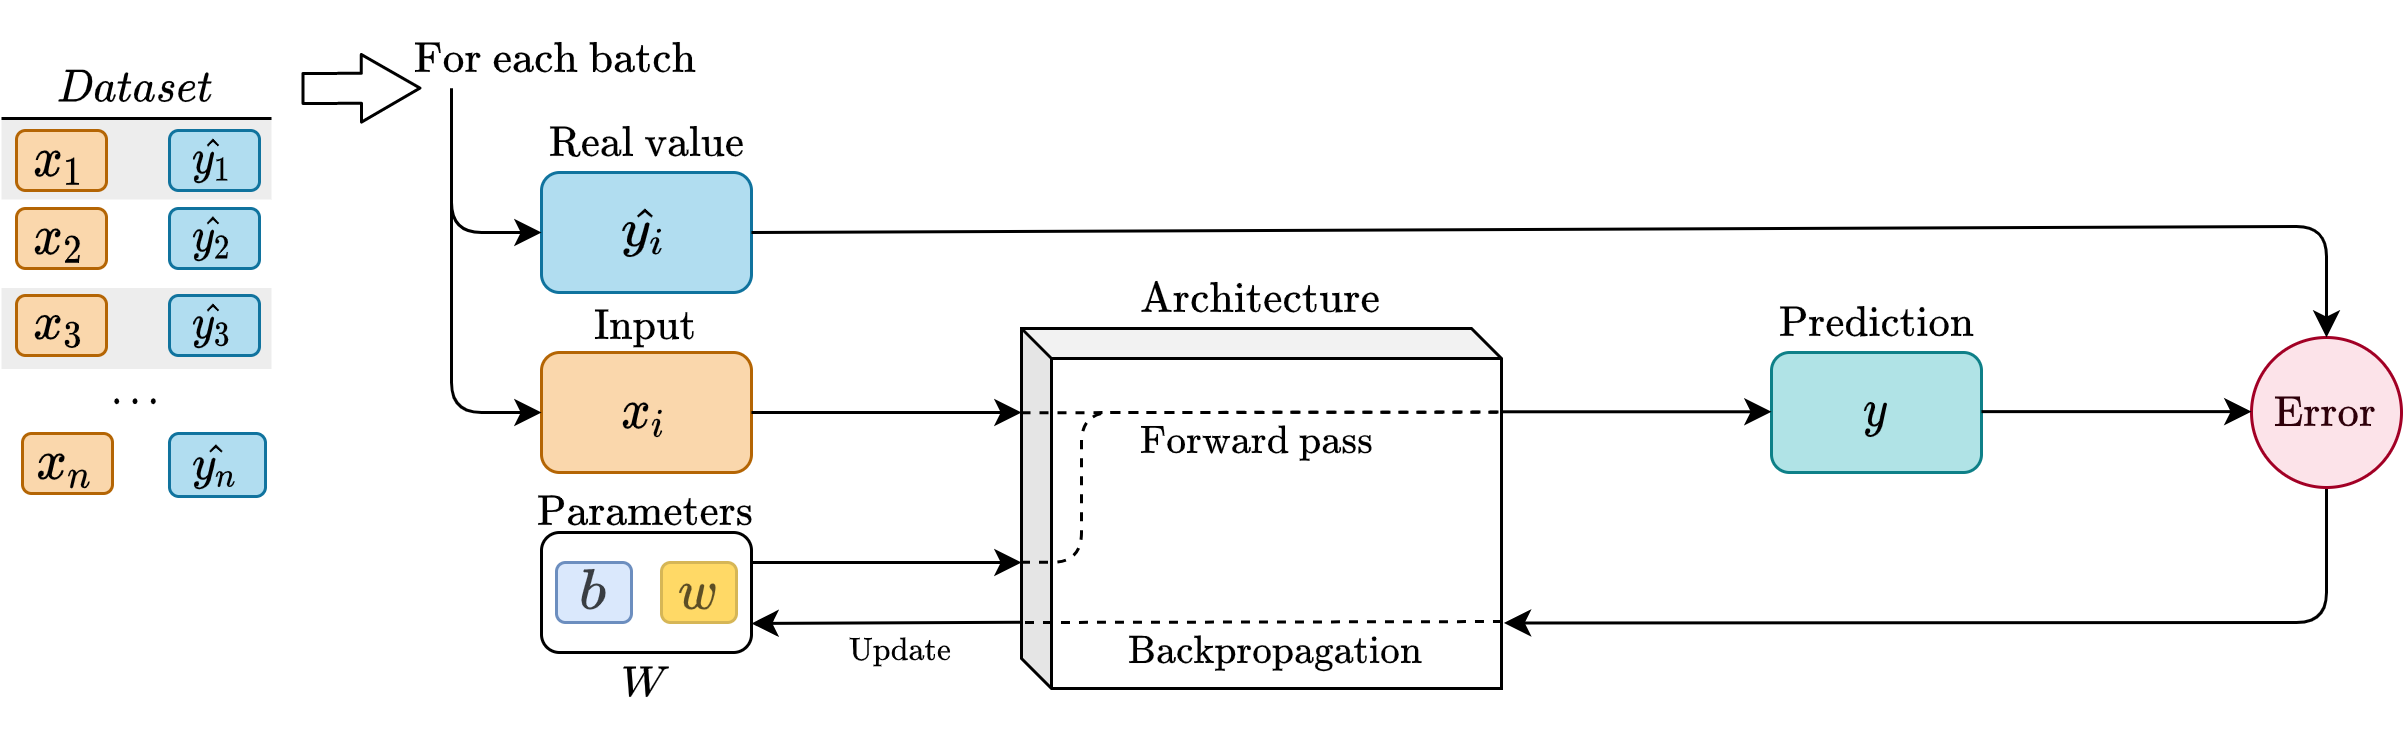
\includegraphics[width=15cm]{images/state-of-art/training/training.png}
    \caption{Proceso de entrenamiento de una red neuronal}
    \label{fig:error_regression}
\end{figure}

\subsubsection{Función de coste}\label{costfunction}
Para que el modelo aprenda es necesario primero saber identificar errores en el proceso. La función de coste es una función que calculará el error que se está produciendo en un modelo. Esta función tendrá dos parámetros: El valor esperado y el valor calculado por el modelo. La diferencia entre ambos valores es lo que se conoce como error o pérdida, por eso esta función también es conocida como función de pérdida o función objetiva. 
\newline

El error más simple es el error dado por la diferencia entre el valor esperado y el valor real:
\newline
\begin{equation}
    \begin{split}
    c_i & = Valor_{real} - Valor_{esperado} = \hat{y_i} - y_i, \\ 
    \text{donde}~c_i &= \text{El valor de la pérdida de la muestra} \\
    i &= \text{i-ésima muestra del \textit{dataset}} \\
    ~\hat{y_i} &= \text{Resultado del modelo} \\
    ~y_i &= \text{Valor real}
  \end{split}
\end{equation}

Usando el ejemplo visto antes en la regresión de la Figura \ref{fig:regression} el error para el dato $i$ visto de forma gráfica sería el siguiente:

\begin{figure}[H]
    \centering
    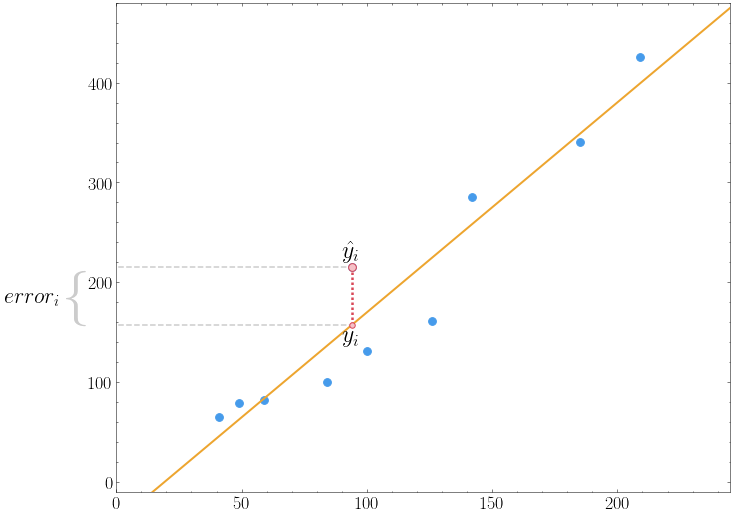
\includegraphics[width=10cm]{images/state-of-art/cost-function/error_function.png}
    \caption{Error de una regresión para el dato $i$}
    \label{fig:error_regression}
\end{figure}


En una red se necesita conocer el error de la capa y no el error de cada neurona. Para ello se aplicará alguna función que reciba un vector como entrada (los errores de cada neurona en una capa) y un único valor de salida (error de la capa). A continuación se listan algunas de las funciones más usadas\cite{tensorflow2015-whitepaper}:


\begin{itemize}
\item Error absoluto medio (\textit{MAE}, siglas en inglés) \cite{errors_basics} \label{MAE_loss}: Es la métrica de error de regresión más simple de entender. Se toma el error absoluto de cada dato, para que los errores negativos y positivos no se anulen. Luego se calculará la media aritmética. En realidad, el \textit{MAE} describe la magnitud típica de los residuos. La ecuación es la siguiente:
\begin{equation}
\centering
    \begin{split}
        \text{MAE} = c_i(y_1, \hat{y_1}) = \frac{1}{n} \sum_{i=1}^n |y_i - \hat{y_i}|
    \end{split}
\end{equation}

\begin{figure}[H]
    \centering
    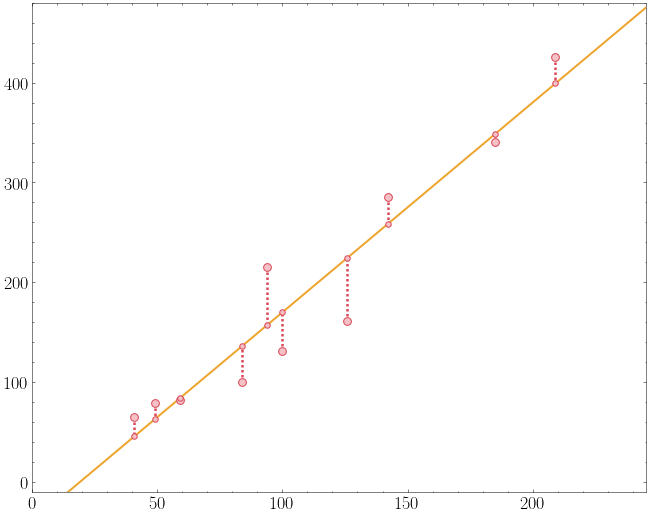
\includegraphics[width=7cm]{images/state-of-art/cost-function/mae.png}
    \caption{Visualización del MAE. El error es la media aritmética de todos los errores.}
    \label{fig:error_mae}
\end{figure}

\item Error cuadrático medio (\textit{MSE}, siglas en inglés) \cite{errors_basics}\label{MSE_loss}: Esta ecuación calcula la media de todos los errores elevados al cuadrado. Elevando al cuadrado se consigue penalizar con mayor intensidad a aquellos puntos que están más alejados de la estimación de la regresión lineal y con menor intensidad a los que se encuentren más cerca. Esta ecuación es muy usada cuando la tarea que se trata de resolver es de tipo regresión. La ecuación es la siguiente:
\begin{equation}
\centering
    \begin{split}
        \text{MSE} = c_i(y_1, \hat{y_1}) &= \frac{1}{n} \sum_{i=1}^n (\sqrt{(\hat{y_i} - y_i)^2}^2) \\
        & = \frac{1}{n} \sum_{i=1}^n (\hat{y_i} - y_i)^2
    \end{split}
\end{equation}

\begin{figure}[H]
    \centering
    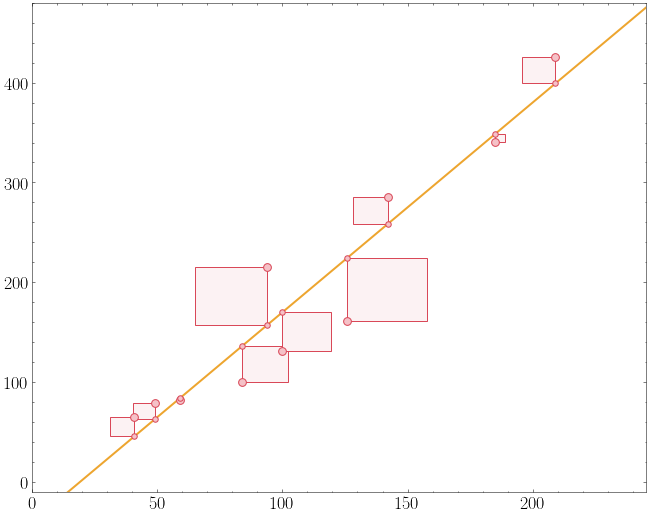
\includegraphics[width=7cm]{images/state-of-art/cost-function/mse.png}
    \caption{Visualización del MSE. El error es la media de las áreas de los cuadrados.}
    \label{fig:error_mae}
\end{figure}

\item Raíz del error cuadrático medio (\textit{RMSE}, siglas en inglés) \cite{errors_basics} \label{RMSE_loss}: Esta ecuación es la raíz cuadrada de \textit{MSE}. Si se compara a nivel de valores, son intercambiables aunque utilizan distinta escala. La ecuación es la siguiente:
\begin{equation}
\centering
    \begin{split}
        \text{MSLE} = \sqrt{MSE} = \sqrt{\frac{1}{n} \sum_{i=1}^n (\hat{y_i} - y_i)^2}
    \end{split}
\end{equation}

\item Error cuadrático medio logarítmico (\textit{MSLE}, siglas en inglés) \cite{errors_basics} \label{MSLE_loss}: Esta ecuación es parecida a \textit{MSE}. Se suele utilizar cuando se sabe previamente que los resultados están normalmente distribuidos y no se quiere que los errores grandes sean significativamente más penalizados que los pequeños. La ecuación es la siguiente:
\begin{equation}
\centering
    \begin{split}
        \text{MSLE} = c_i(y_1, \hat{y_1}) &= \frac{1}{n} \sum_{i=1}^n (\log{y_i + 1} - \log{\hat{y_i} + 1}) \\
        & = \frac{1}{n} \sum_{i=1}^n \left(\log{\left(\frac{y_i + 1}{\hat{y_i} + 1}\right)}\right)^2
    \end{split}
\end{equation}


\item Pérdida de \textit{Huber}\cite{huber_loss}\label{huber_loss}: Ya se sabe que el Error Medio Cuadrado (\textit{MSE}) es mejor para aprender los valores atípicos en el conjunto de datos, por otro lado, el Error Medio Absoluto (\textit{MAE}) es bueno para ignorar los valores atípicos. Pero en algunos casos, los datos que parecen atípicos no molestan y no deberían tener alta prioridad. La pérdida de Huber es una combinación \textit{MSE} y \textit{MAE}. Se usará $\delta$ para definir un sesgo para usar \textit{MAE} o \textit{MSE}. La ecuación es la siguiente:
\begin{equation}
\centering
    \begin{split}
    \text{Huber\_loss} = c_i(y_1, \hat{y_1}) &= \left\{ 
        \begin{array}{cl} 
            MSE & \text{si }|\hat{y}-y| \le \delta, \\
            MAE & \text{e.o.c.}
        \end{array}\right. \\ &= \left\{ 
        \begin{array}{cl} 
            \frac{1}{n} \sum_{i=1}^n (\hat{y_i} - y_i)^2 & \text{si }|\hat{y}-y| \le \delta, \\
            \delta \left(\frac{1}{n} \sum_{i=1}^n |y_i - \hat{y_i}|-\frac{\delta}{n}\right) & \text{e.o.c.}
        \end{array}\right.
    \end{split}
\end{equation}

\begin{figure}[H]
    \centering
    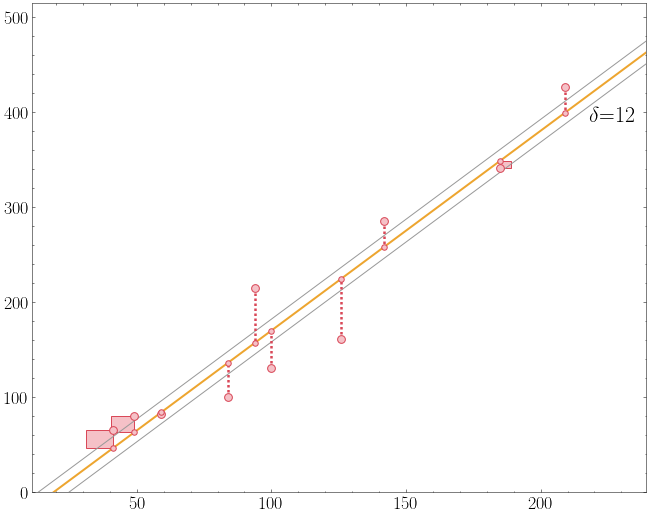
\includegraphics[width=7cm]{images/state-of-art/cost-function/huber.png}
    \caption{Visualización de la pérdida de Huber. Se calcula \textit{MSE} si $|\hat{y}-y| \le \delta$, en otro caso se calcula \text{MAE}.}
    \label{fig:error_mae}
\end{figure}


\item Error medio porcentual absoluto (\textit{MAPE}, siglas en inglés)\cite{errors_basics} \label{MAPE_loss}: Es el porcentaje equivalente de \textit{MAE}. La ecuación es igual a la de \textit{MAE}, pero con ajustes para convertir los valores en porcentajes. Permiten ver la distancia entre los resultados del modelo y el resultado real mostrando el dato de manera más fácil de interpretar para los seres humanos. La ecuación es la siguiente:
\begin{equation}
\centering
    \begin{split}
        \text{MAPE} = c_i(y_1, \hat{y_1}) &= \frac{100\%}{n} \sum_{i=1}^n \left|\frac{y_i-\hat{y_i}}{y}\right|
    \end{split}
\end{equation}

\begin{figure}[H]
    \centering
    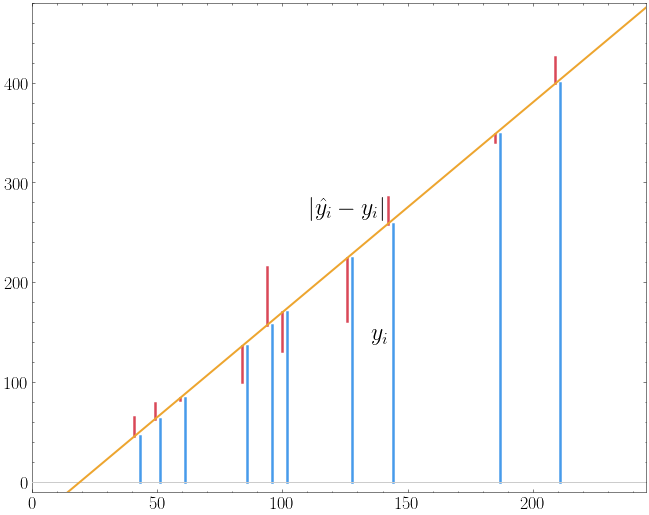
\includegraphics[width=7cm]{images/state-of-art/cost-function/mape.png}
    \caption{Visualización del MAPE. El error es la media de las proporciones de los errores respecto al valor $y$.}
    \label{fig:error_mae}
\end{figure}

\item Porcentaje medio de error (\textit{MPE}, siglas en inglés)\cite{errors_basics} \label{MPE_loss}: Es exactamente que \textit{MAPE}, pero sin el valor absoluto. Dado que los errores positivos y negativos se anulan, no se puede hacer ninguna declaración sobre el rendimiento general de las predicciones del modelo. Sin embargo, si hay más errores negativos o positivos, este sesgo se mostrará en el \textit{MPE}. A diferencia del \textit{MAE} y del \textit{MAPE}, el \textit{MPE} es útil porque permite ver si el modelo sistemáticamente subestima (más errores negativos) o sobreestima (errores positivos). La ecuación es la siguiente:
\begin{equation}
\centering
    \begin{split}
        \text{MPE} = c_i(y_1, \hat{y_1}) &= \frac{100\%}{n} \sum_{i=1}^n \frac{y_i-\hat{y_i}}{y}
    \end{split}
\end{equation}

\begin{figure}[H]
    \centering
    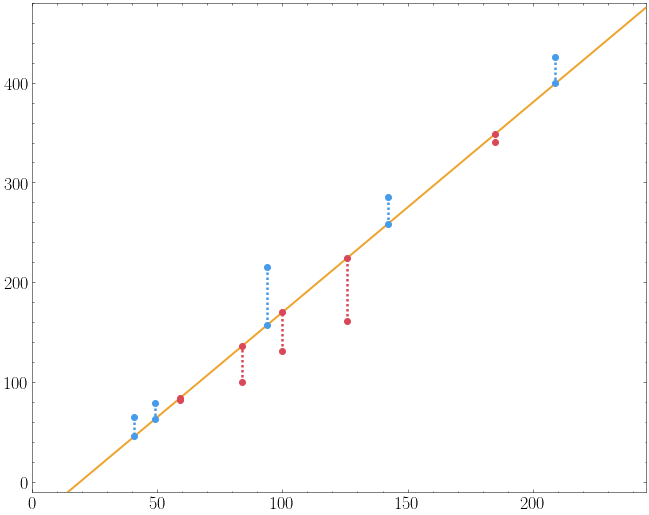
\includegraphics[width=7cm]{images/state-of-art/cost-function/mpe.png}
    \caption{Visualización del MPE. Muestra la cantidad de errores que son positivos y la cantidad que son negativos.}
    \label{fig:error_mae}
\end{figure}


\item Pérdida de entropía cruzada: Se utiliza explícitamente para comparar una probabilidad de "verdad fundamental" ($y$ u "objetivos") y alguna distribución predicha ($\hat{y}$ o "predicciones"). Tiene como objetivo calcular la media de las probabilidades de que un valor pertenece a una clase o a otra, por lo que es muy útil para problemas de clasificación. Es muy usada cuando se usa la función de activación \textit{softmax}, puesto que esta, también trabaja con probabilidades.
\begin{equation}
\centering
    \begin{split}
        c_i(y_1, \hat{y_1}) &= - \sum_i y_{i,j}log(\hat{y_{i,j}})\\
        \text{donde}~j &= \text{Índice de la probabilidad "verdadera"}
    \end{split}
\end{equation}

La probabilidad "verdadera" es un vector con todos los valores a $0$ excepto uno de ellos que tiene el valor igual a $1$. Este tipo de vector es conocido como vector \textit{one-hot}, donde un valor es \textit{hot} si es igual a $1$ o \textit{cold} si es igual a 0. Cuando se comparan los resultados del modelo con un vector \textit{one-hot} usando la entropía cruzada, los valores igual a $0$ no se usan, y la pérdida de logaritmo de la probabilidad del objetivo se multiplica por $1$, haciendo que el cálculo de la entropía cruzada sea relativamente simple. Este es también un caso especial del cálculo de la entropía cruzada, llamado entropía cruzada por categorías. 
\newline

Un ejemplo de un vector \textit{one-hot} sería el siguiente: $[0,1,0,0]$ donde por ejemplo se representarían las siguientes clases: Perro, gato, caballo y elefante. El $1$ representa que el dato dado al modelo representa a un gato. Este tipo de vectores se usan mucho en tareas de clasificación y en \textit{NLP}.
\newline

Hay un subtipo denominado pérdida de entropía cruzada binaria. Este tipo de error se puede calcular cuando se intenta clasificar solo con dos tipos: $0$ o $1$. Normalmente se usa como si fuese un valor booleano en un lenguaje de programación. Un \verb|true| si es del tipo A o un \verb|false| si no es del tipo A. Por ejemplo: gato o no gato o en interior o en exterior. La ecuación matemática es la siguiente:
\begin{equation}
\centering
    \begin{split}
        c_{i,j}(y_1, \hat{y_1}) &= (y_{i,j})(-log(\hat{y}_{i,j})) + (1-y_{i,j}) (-log(1 - \hat{y}_{i,j})) \\
        &= -y_{i,j} \cdot log(\hat{y}_{i,j}) - (1 - y_{i,j}) \cdot log(1 - \hat{y}_{i,j})
    \end{split}
\end{equation}


\end{itemize}


\subsubsection{Minimizando el error}\label{minimizing-error}

Una vez elegida alguna de las funciones de coste, el objetivo es minimizar el error y así mejorar el modelo:

\begin{equation}
\begin{split}
        W^* &= \argmin_{W} \frac{1}{n} \sum_{i=1}^n c(a(x^{(i)}; W), y^{(i)}) \\
        &= \argmin_{W} c_i(W) \\
        \text{donde}~x^{(i)} &= \text{Vector de entrada para el dato }i \\
        y^{(i)} &= \text{Vector real para el dato }i \\
        W &= \text{Matrices con los pesos y bias de cada cada} 
  \end{split}
\end{equation}

Para calcular el mínimo de una función, se necesita calcular la derivada de dicha función e igualarla a 0. Minimizando la función de coste, es decir, derivando la función de coste, también se minimiza el error. Para ello hay distintas formas de minimizar el error:
\begin{itemize}
\item Minimizar función de coste

Este fue el algoritmo usado en las redes de perceptrones para calcular la matriz $W$. El funcionamiento de este algoritmo es sencillo. Partiendo de la definición de una función de coste cualesquiera que permita cuantificar el error del modelo, se tratará de minimizar dicho valor. Una de las ecuaciones más populares es la que se conoce como el Mínimo de Cuadrados Ordinarios. Esta función parte de la derivada de \textit{MSE}:

\begin{equation}
    \begin{split}
    L_i & =  (\hat{y_i} - y_i)^2 \\
     & = (y - x \cdot W)' \cdot (y - x \cdot W) \\
     & = y'y - W'x'y - y'xW + W'x'x W
  \end{split}
\end{equation}

Derivando y despejando:
\begin{equation}
    \begin{split}
L_i'() = & -2x'y + 2x'xW \\
W^* = & (x'x)^{-1}x'y
\end{split}
\end{equation}

Esta ecuación permite el cálculo de la matriz $W$ óptima posible solo usando los valores de entrada y de salida de modelo como argumentos. Aunque este algoritmo de entrenamiento tiene varias limitaciones:
\begin{itemize}
\item No es extensible a redes más complejas.
\item El cálculo de la matriz inversa es muy costoso computacionalmente.
\item Se ha usado el error mínimo cuadrado, una de las más simple, puesto que es una función con forma convexa y por tanto una derivada fácil de calcular, pero hay otras funciones de coste que no permiten minimizar el error con esta técnica.
\newline

Estas limitaciones, demostradas matemáticamente en el libro "\textit{Perceptron}"\cite{papert} de Minsky y Papert (1969), provocó un corte repentino en la financiación de proyectos de inteligencia artificial y más específicamente en aquellos relacionados con los sistemas de redes neuronales durante un periodo de más de 15 años conocidos como el invierno de la inteligencia artificial.
\end{itemize}


\item Descenso del gradiente

Este algoritmo no es una fórmula como los mínimos cuadrados ordinarios, sino un método iterativo que poco a poco va minimizando el error. De algún modo se puede asimilar a como aprendemos los seres humanos: No con una única fórmula, sino a través de la experiencia reduciendo nuestros errores con el tiempo.
\newline

El cálculo del gradiente es un proceso que se puede representar de la siguiente forma:
\begin{figure}[H]
    \centering
    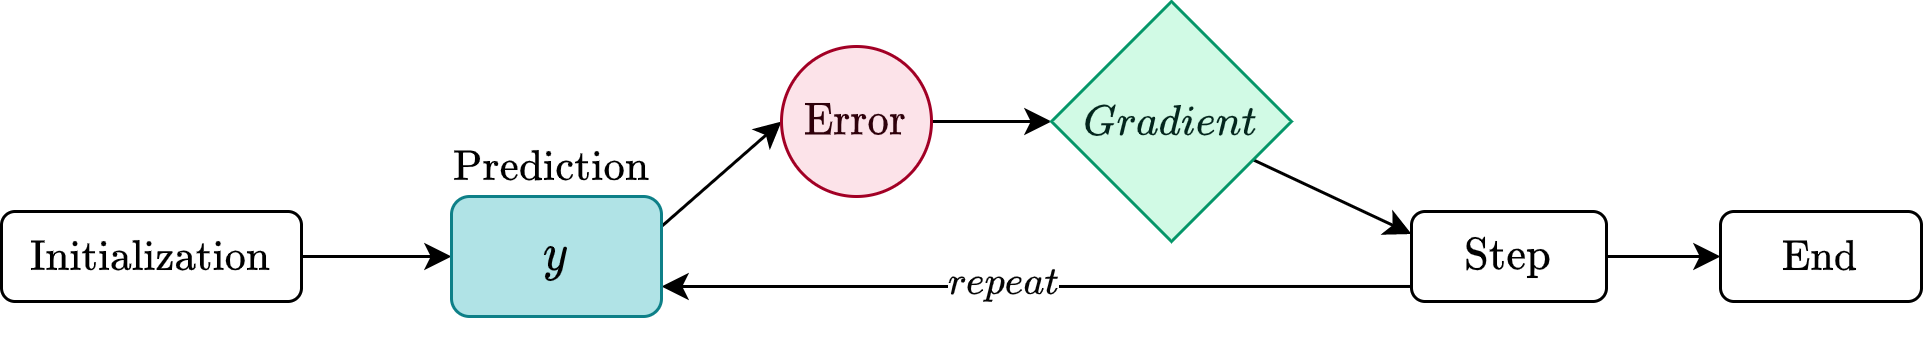
\includegraphics[width=13cm]{images/state-of-art/gradient-descent/gradient-algorithm.png}
    \caption{Proceso iterativo para minimizar el error}
    \label{fig:gradient_descent}
\end{figure}

El método de los Mínimos Cuadrados Ordinarios minimiza el error igualando la derivada a $0$ para poder hallar los mínimos de \textit{MSE}. Con esto, se pueden calcular los mínimos locales y globales, pero también se puede calcular máximo locales, puntos de inflexión o puntos de silla provocando un sistema de ecuaciones grande y bastante ineficiente de resolver \cite{papert}.
\newline

Una forma de entender este método es el siguiente: Una persona se encuentra en un terreno montañoso y el objetivo de esta persona es llegar al punto más bajo. Para ello, analizará el terreno donde se encuentra y evaluará la pendiente y se moverá hacia donde la pendiente desciende con mayor intensidad. Descenderá una cantidad de pasos y repetirá el proceso: analizar la inclinación y descender. Esto se repetirá hasta que llegué a lo más abajo posible y no haya forma alguna de seguir bajando. Esta es la lógica del algoritmo del descenso del gradiente.

\begin{figure}[H]
    \centering
    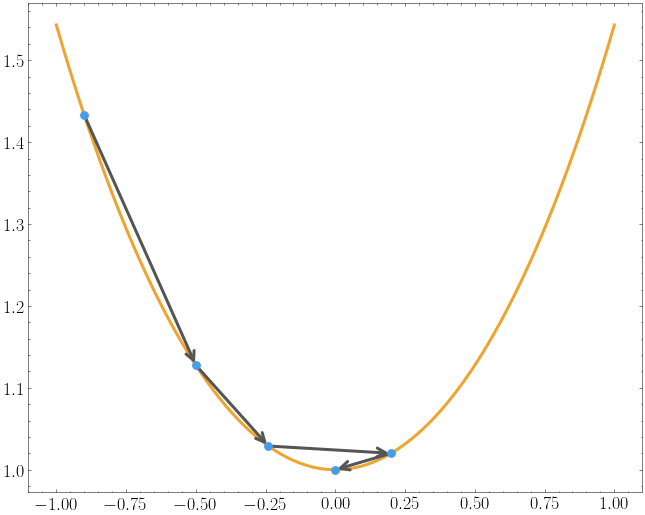
\includegraphics[width=7cm]{images/state-of-art/gradient-descent/gradient.png}
    \caption{Ejemplo gráfico de la iteración del descenso del gradiente}
    \label{fig:gradient_descent}
\end{figure}


El terreno en esta metáfora sería la función de coste. La persona es el valor calculado por la función de coste, el cual se quiere minimizar y por ello se evalúa la pendiente o gradiente solo en ese punto y de ese modo no se depende de la derivada de la función de coste sino de la derivada parcial respecto a cada uno de los valores de entrada en la neurona. El número de pasos que la persona bajará es un valor conocido como tasa de aprendizaje (\textit{learning rate} en inglés) y es un parámetro más de la red neuronal. 
\newline


En la figura \ref{fig:gradient_descent}, hay dos ejes, representando una neurona que tiene solo un argumento de entrada. El eje de ordenadas representa el error de la neurona. Se ha representado un espacio bidimensional, pero se puede usar cualquier dimensión puesto que el número de entradas de la neurona no está limitado. Usando un espacio tridimensional, la función de coste sería una superficie irregular. De hecho, el vector $\nabla f$ siempre tendrá como mínimo dos valores, un peso $w$ y la bias $b$.
\newline

En este trabajo no se explica cómo calcular la derivada de una función o derivada parcial($\sigma$). Dicho esto, matemáticamente, el proceso de este algoritmo es el siguiente \cite{}:
\begin{enumerate}
\item Se inicializa los pesos $w$ y bias $b$ de la neurona quieren ajustar de forma aleatoria:
\begin{equation}
    ~N(0, \sigma_2)
\end{equation}

\item Se realiza un bucle hasta la convergencia:
\begin{enumerate}

\item Se calculan derivadas parciales para cada uno de los parámetros. Una derivada parcial mide cuanto impacto tiene una única variable de entrada en la salida de la función y se calcula igual que una derivada, lo único que se repite la derivada para cada variable de entrada. Cada uno de esos valores indicará cual es la pendiente en el eje de dicho parámetro relacionado a un único valor de entrada.

\begin{equation}
    \begin{split}
    \nabla f &= \nabla f_b \oplus \nabla f_w \\\
    \nabla f_b &= \begin{pmatrix} \frac{\partial c}{\partial b} \end{pmatrix}\\
    \nabla f_w &= \begin{pmatrix} \frac{\partial c}{\partial w_1}, & \frac{\partial c}{\partial w_2}, & \cdots , &  \frac{\partial c}{\partial w_n} \end{pmatrix}
  \end{split}
  \label{eqn:gradients}
\end{equation}


Conjuntamente todas las direcciones, es decir, todas las derivadas parciales conforman un vector que indica la dirección a la que la pendiente asciende, este vector es también conocido como gradiente($\nabla f$) y el cual tendrá el mismo número de elementos que el vector de entrada y cada valor contendrá la solución a la derivada parcial con respecto a cada uno de los valores de entrada.
\newline

El objetivo de esta función es minimizar y no maximizar, por lo que se negará el gradiente para indicar la dirección en la que la pendiente desciende.

\begin{equation}
    \nabla f = -\nabla f_b \oplus \nabla f_w
\end{equation}

\item Se actualizan los pesos con los nuevos valores del gradiente negativo multiplicado por la tasa de aprendizaje. La tasa de aprendizaje es simplemente un valor que determina como de grande será el paso en cada iteración que se verá con mayor profundidad en la sección \ref{learningrate}:
\begin{equation}
    \begin{split}
    b^* = b - \eta * \nabla f_b \\
    w^* = w - \eta * \nabla f_w
    \end{split}
\end{equation}

Al igual que ocurría con el algoritmo de \textit{feed-forward}, el descenso del gradiente trabajará por capas, por lo que este último paso se debería representar de la siguiente forma:

\begin{equation}
    W^* = W - \eta * \nabla f
\end{equation}

Esta ecuación representa que se actualizarán los pesos de todas las neuronas en una capa.

\end{enumerate}
\end{enumerate}

Este método se aplicará a todas las neuronas de la red. Dado un error, el descenso del gradiente obtendrá un vector que contendrá la derivada de los parámetros respecto al coste. Es decir, el gradiente será un vector con distintos valores, cuanto más grande sea dicho valor, más corrección se debe aplicar al parámetro que corresponde. Visto gráficamente se puede ver de la siguiente forma:

\begin{figure}[H]
    \centering
    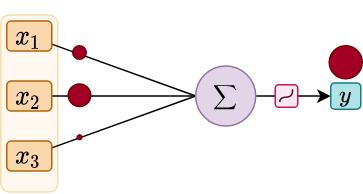
\includegraphics[width=7cm]{images/state-of-art/gradient-descent/gradient_diagram.png}
    \caption{Representación del descenso del gradiente en una neurona. Lo rojo es la representación del error.}
    \label{fig:gradient_descent}
\end{figure}

Las derivadas parciales que se deben resolver para obtener el vector gradiente $\nabla f$, indica como varía el coste ante el cambio de los parámetro $w$ y $b$. A continuación, se muestra una imagen de las distintas partes de las derivadas parciales:

\begin{figure}[H]
    \centering
    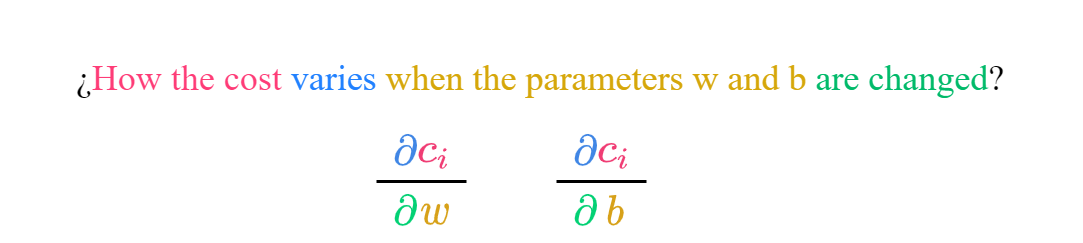
\includegraphics[width=13cm]{images/state-of-art/gradient-descent/dx.png}
    \caption{Derivadas parciales usadas en el descenso del gradiente.}
    \label{fig:gradient_descent}
\end{figure}

\end{itemize}



\subsubsection{Backpropagation}\label{backpropagation}

En 1986, Rumelhart junto con otros investigadores publicaron “Learning representation by back-propagating errors” \cite{rumelhart}, un trabajo que volvió dar popularidad a las redes neuronales. El trabajo, basado en otros trabajos basados en diferenciación automáticas mostró experimentalmente como usando un nuevo algoritmo de aprendizaje se podría conseguir que una red neuronal se auto ajustará sus parámetros para así aprender una representación interna de la información que estaba procesando, un algoritmo conocido como \textit{backpropragation}.
\newline

Este algoritmo es adaptable a cualquier modelo y con él, dio por finalizado lo que históricamente se conoce como Invierno de la IA consiguiendo nuevas financiaciones y nuevos proyectos en el campo del \textit{Deep Learning}.
\newline

La predicción de un modelo se obtiene usando un algoritmo llamado \textit{feed-forward} como se ha explicado en la Sección \ref{feedforward}. Dicho valor debe ajustarse lo mejor posible al valor real. Para ello, se debe ir ajustando en un método iterativo las matrices $W$ en un proceso que se conoce como entrenamiento (ver Sección \ref{training}). En cada iteración del entrenamiento se irá ajustando las matrices $W$ haciendo uso primero de la función de coste, que mostrará la magnitud del error (ver Sección \ref{costfunction}), posteriormente ese error se irá propagando hacia atrás en el modelo para conocer la responsabilidad de cada neurona usando un algoritmo conocido como \textit{backpropagation} y finalmente, por cada neurona se calculará el vector gradiente $\nabla f$ que representa como ha afectado la neurona al resultado final y con ello se ajustarán sus distintos pesos $w$ y bias $b$(ver Sección \ref{minimizing-error}). 
\newline

El algoritmo de \textit{backpropagation} se puede representar gráficamente:

\begin{figure}[H]
    \centering
    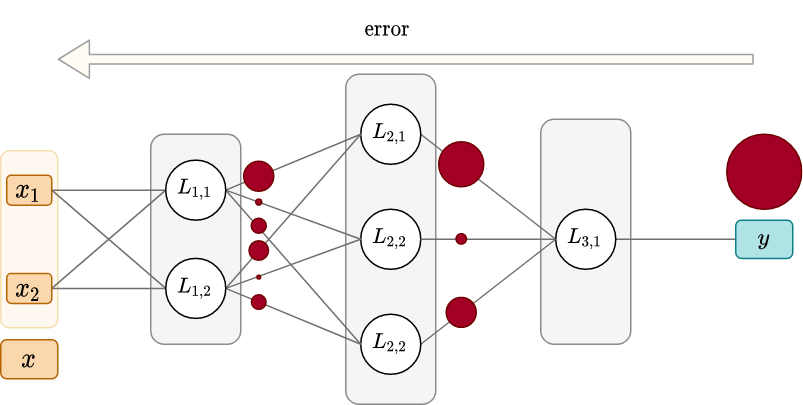
\includegraphics[width=14cm]{images/state-of-art/back-propagation/network_descent_gradient.png}
    \caption{Representación del algoritmo de backpropagation.}
    \label{fig:basic_network}
\end{figure}

En esta red se representa con círculos rojos el error de cada neurona. El error calculado por la función de coste es el error más grande que es el que está relacionado con la salida del modelo. A partir de ese punto, se retropropagará hacia atrás y se computará que parte del error pertenece a cada neurona hasta la primera capa. Por ejemplo, en la capa $L_2$, la principal neurona que tiene parámetros desajustados es $L_{2,1}$. A su vez, ese error principalmente tiene parte de la culpa debido a la neurona $L_{1,1}$. Por lo tanto, es lógico pensar que habría que ajustar neuronas como $L_{2,1}$ o $L_{1,1}$, sin embargo, dejar tal como están neuronas como $L_{1,2}$ o $L_{2,2}$.
\newline
 
A continuación, se define la red neuronal más simple que se puede construir con una sola neurona oculta y una neurona de salida.
\begin{figure}[H]
    \centering
    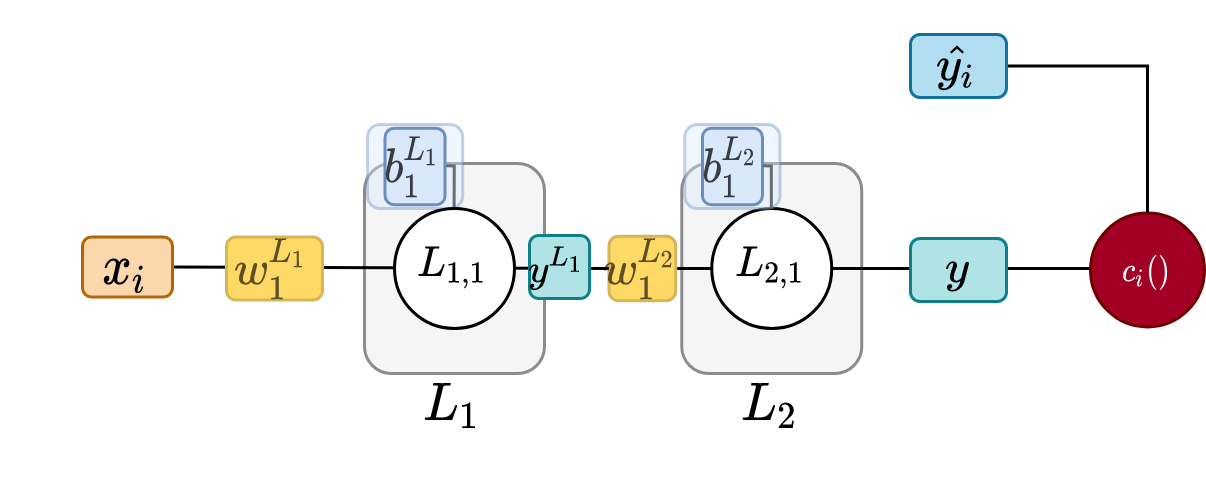
\includegraphics[width=12cm]{images/state-of-art/back-propagation/basic_network.png}
    \caption{Red neuronal básica.}
    \label{fig:basic_network}
\end{figure}

Para realizar el algoritmo de \textit{backpropagation}, primero se debe de computar la pérdida con la función $c_i$. Posteriormente, el algoritmo de \textit{backpropagation} "distribuirá" la pérdida del modelo a las capas anteriores (siempre se empieza por la última capa). Esta computación expresa cómo de importante son las matrices $W$ indicando cuánto impacto tiene en el modelo. Por ejemplo, si se cambia algún valor de $W_2$ de alguna forma, se podrá saber cómo afecta al resultado de la predicción del modelo. Matemáticamente:

\begin{equation}
\begin{split}
    \frac{\partial c}{\partial w^{L_2}} &= \frac{\partial c(a(z^{L_2}))}{\partial w^{L_2}} \\
    \frac{\partial c}{\partial b^{L_2}} &= \frac{\partial c(a(z^{L_2}))}{\partial b^{L_2}} 
    \label{eqn:backpropagationsimplenetworklayer2}
\end{split}
\end{equation}

El numerador es una composición de funciones, y es básicamente el cálculo del algoritmo \textit{feed-forward}(ver sección \ref{feedforward}). Para calcular la derivada parcial de una composición de funciones, hay que hacer uso de una herramienta de cálculo conocida como la regla de la cadena (\textit{chain rule}).
\newline

Un ejemplo para entender la \textit{chain rule} sería el siguiente. Se sabe que el Sol es $100$ veces más grande que la Tierra. A su vez, la Tierra es $4$ veces más grande que la Luna. Sabiendo esas dos relaciones, se puede saber cuánto es el Sol más grande que la Luna. Para ello simplemente multiplicamos $100 \times 4 = 400$. El sol por lo tanto es $400$ veces más grande que la Luna. Definiendo este problema con ecuaciones:

\begin{equation}
\begin{split}
    \frac{\partial T_{\text{Sol}}}{\partial T_{\text{Tierra}}} = 100
    \qquad
    \frac{\partial T_{\text{Tierra}}}{\partial T_{\text{Luna}}} = 4 \\
    \frac{\partial T_{\text{Sol}}}{\partial T_{\text{Luna}}} = \frac{\partial T_{\text{Sol}}}{\partial T_{\text{Tierra}}} \cdot \frac{\partial T_{\text{Tierra}}}{\partial T_{\text{Luna}}} = 400 \nonumber
\end{split}
\end{equation}

Se le llama la \textit{chain rule} porque se encadena en relación con el dato en común, en este caso $T_\text{Tierra}$ es la parte común que en un lado se encuentra en el denominador y en otro en el numerador. Por lo tanto, para derivar la composición de funciones vista en la Ecuación \ref{eqn:backpropagationsimplenetworklayer2}, simplemente hay que multiplicar cada una de las derivadas intermedias. Recordando las ecuaciones del algoritmo de \textit{feed-forward} y la composición de funciones para calcular el error del modelo para la red mostrada en la Figura \ref{fig:basic_network}:

\begin{equation}
\begin{split}
    z^{L_2} = W^{L_2} \cdot y^{L_1} + b^{L_2}
    \qquad
    c(a^{L_2}(z^{L_2}))
\end{split}
\end{equation}

Se calcula como se propaga el error de la capa $L_2$ a la capa $L_1$:

\begin{equation}
\begin{split}
     \frac{\partial c}{\partial w^{L_2}} &= \frac{\partial c}{\partial a^{L_2}} \cdot \frac{\partial a^{L_2}}{\partial z^{L_2}} \cdot \frac{\partial z^{L_2}}{\partial w^{L_2}} \\
     \frac{\partial c}{\partial b^{L_2}} &= \frac{\partial c}{\partial a^{L_2}} \cdot \frac{\partial a^{L_2}}{\partial z^{L_2}} \cdot \frac{\partial z^{L_2}}{\partial b^{L_2}}
\end{split}
 \label{eqn:backpropagationlayer2}
\end{equation}

Estas derivadas son fáciles de calcular y la explicación de cada derivada sería la siguiente:

\begin{itemize}
\item 1º derivada. Derivada de la función de activación respecto al coste:

\begin{equation}
    \frac{\partial c}{\partial a^{L_2}}
\end{equation}

Como varia el coste de la red (es la última capa) cuando se varía la salida de la función de activación de la red. En otras palabras, se calcula la derivada de la función de coste con respecto a la salida de la red neuronal. Es necesario, por tanto, saber la derivada de la función de coste usada.

\item 2º derivada. Derivada de la activación respecto a $z$:
\begin{equation}
    \frac{\partial a^{L_2}}{\partial z^{L_2}}
\end{equation}

Trata de reflejar como varía la salida de la neurona cuando se varía la suma ponderada de la neurona. La derivada que hay que usar es la derivada de la función de activación que se pueden ver en la sección \ref{activationfunction}. Derivada de la suma ponderada respecto a los valores de los pesos y bias.

\item 3º derivada: Derivada de $z$ respecto a los parámetros:
\begin{align*}
    \frac{\partial z^{L_2}}{\partial w^{L_2}} && \frac{\partial z^{L_2}}{\partial b^{L_2}}
\end{align*}

Indica como varía la suma ponderada $z$ con respecto a una variación de los parámetros. El parámetro $b$ es un valor independiente por lo que su derivada es una constante igual a $1$. Por otro lado, la derivada $\frac{\partial z^{L_2}}{\partial w^{L_2}}$ depende de la anterior capa.

\begin{align*}
    \frac{\partial z^{L_2}}{\partial w^{L_2}} = a^{L_1} && \frac{\partial z^{L_2}}{\partial b^{L_2}} = 1
\end{align*}

\end{itemize}

Partiendo de esta definición, se puede unir la 1º y 2º derivada en una sola:

\begin{equation}
     \frac{\partial c}{\partial a^{L_2}} \cdot \frac{\partial a^{L_2}}{\partial z^{L_2}} = \frac{\partial c}{\partial z^{L_2}}
\end{equation}

Esta derivada indica en qué grado se modifica el error cuando se produce un cambio en el error cuando se produce un pequeño cambio en la suma de las neuronas de la capa. Si el valor es grande es que ante un pequeño cambio en cualquiera de las neuronas de las capas en el valor $z$, se verá reflejado en el resultado del modelo. Por el contrario, si el valor es pequeño, un gran cambio en cualquiera de las neuronas en el valor de $z$ de no afectará al resultado final. En resumen, esta derivada muestra cómo afecta la capa (o alguna neurona en especial puesto que es un vector) en el resultado final y por lo tanto al error de la red y de esa forma el algoritmo del descenso del gradiente modificará los parámetros para poder obtener el mejor resultado posible. A esta derivada también se le conoce como el error imputado a la capa y se representa con $\delta$:  

\begin{equation}
    \frac{\partial c}{\partial a^{L_2}} \cdot \frac{\partial a^{L_2}}{\partial z^{L_2}} = \frac{\partial c}{\partial z^{L_2}} = \delta^{L_2}
\end{equation}

Con esta nueva definición, se puede reescribir la Ecuación \ref{eqn:backpropagationlayer2} de la siguiente forma:

\begin{equation}
\begin{split}
     \frac{\partial c}{\partial w^{L_2}} &= \frac{\partial c}{\partial a^{L_2}} \cdot \frac{\partial a^{L_2}}{\partial z^{L_2}} \cdot \frac{\partial z^{L_2}}{\partial w^{L_2}} \\ &= \delta^{L_2} \cdot \frac{\partial z^{L_2}}{\partial w^{L_2}} = \delta^{L_2} \cdot a^{L_1}
\end{split}
\label{eqn:backpropagation_b}
\end{equation}

\begin{equation}
\begin{split}
     \frac{\partial c}{\partial b^{L_2}} &= \frac{\partial c}{\partial a^{L_2}} \cdot \frac{\partial a^{L_2}}{\partial z^{L_2}} \cdot \frac{\partial z^{L_2}}{\partial b^{L_2}} \\ &= \delta^{L_2} \cdot \frac{\partial z^{L_2}}{\partial b^{L_2}} = \delta^{L_2} \cdot 1
\end{split}
\label{eqn:backpropagation_w}
\end{equation}

Pero el modelo no solo depende de la segunda capa y de $W_2$, también depende de la primera capa y de $W_1$. Es aquí donde mana la belleza del algoritmo de \textit{backpropagation}. El error se puede retropropagar de manera similar usando el mismo razonamiento. Primero se muestran la composición de funciones:

\begin{equation}
\begin{split}
    \frac{\partial c}{\partial w^{L_1}} &= \frac{\partial c(a(z^{L_2}(a(z^{L_1}))))}{\partial w^{L_2}} \\
    \frac{\partial c}{\partial b^{L_1}} &= \frac{\partial c(a(z^{L_2}(a(z^{L_1}))))}{\partial b^{L_2}} 
    \label{eqn:backpropagationsimplenetworklayer2}
\end{split}
\end{equation}

Usando la \textit{chain rule} se divide en distintas partes:

\begin{equation}
\begin{split}
     \frac{\partial c}{\partial w^{L_1}} &= \frac{\partial c}{\partial a^{L_2}} \cdot \frac{\partial a^{L_2}}{\partial z^{L_2}} \cdot \frac{\partial z^{L_2}}{\partial a^{L_1}} \cdot \frac{\partial a^{L_1}}{\partial z^{L_1}} \cdot \frac{\partial z^{L_1}}{\partial x} \\
     \frac{\partial c}{\partial b^{L_1}} &= \frac{\partial c}{\partial a^{L_2}} \cdot \frac{\partial a^{L_2}}{\partial z^{L_2}} \cdot \frac{\partial z^{L_2}}{\partial a^{L_1}} \cdot \frac{\partial a^{L_1}}{\partial z^{L_1}} \cdot \frac{\partial z^{L_1}}{\partial 1} \\
\end{split}
 \label{eqn:backpropagationlayer1}
\end{equation}


En realidad, de las $6$ derivadas mostradas, sólo haría falta calcular una de ellas. Las derivadas $\frac{\partial c}{\partial a^{L_2}} \cdot \frac{\partial a^{L_2}}{\partial z^{L_2}} $ ya han sido calculadas y son igual a $\delta^{L_2}$. En cuanto a la derivada $\frac{\partial z^{L_1}}{\partial x}$, simplemente es obtener el resultado de la anterior capa o bien usar $x$ si es la primera capa como es este caso. La derivada $\frac{\partial z^{L_1}}{\partial 1}$ es un valor constante por lo que no pasa nada. Finalmente, la derivada $\frac{\partial a^{L_1}}{\partial z^{L_1}}$ es simplemente la derivada de la función de activación de dicha capa. Es por esta razón por lo que en la sección \ref{activationfunction} se explicaba que es mejor usar una única función de activación para toda la capa y así poder facilitar los cálculos.
\newline

La única derivada que queda por explicar es $\frac{\partial z^{L_2}}{\partial a^{L_1}}$ la cual expresa como varía la suma ponderada de una capa cuando se varía el vector de entrada de dicha capa. El cálculo de esta derivada es simplemente la matriz de parámetros $W^{L_1}$ que conecta ambas capas. Básicamente, esta derivada mueve el error de la capa $L_2$ a la capa $L_1$ distribuyendo el error en función de las ponderaciones de las conexiones. Al igual que se hizo con la anterior capa, con esta capa también se puede definir el error imputado:


\begin{equation}
   \frac{\partial c}{\partial a^{L_1}} = \frac{\partial c}{\partial a^{L_2}} \cdot \frac{\partial a^{L_2}}{\partial z^{L_2}} \cdot \frac{\partial z^{L_2}}{\partial a^{L_1}} \cdot \frac{\partial a^{L_1}}{\partial z^{L_1}} = \delta^{L_1}
\end{equation}

Por lo tanto, la Ecuación \ref{eqn:backpropagationlayer1} quedaría de la siguiente forma:
\begin{equation}
\begin{split}
     \frac{\partial c}{\partial w^{L_1}} &= \delta^{L_1} \cdot \frac{\partial z^{L_1}}{\partial x} \\
     \frac{\partial c}{\partial b^{L_1}} &= \delta^{L_1} \frac{\partial z^{L_1}}{\partial 1} \\
\end{split}
\end{equation}

En resumen, se ha podido explicar cómo propagar el error a cualquier capa de la red y calcular la derivada respecto a los parámetros con las siguientes ecuaciones:

\begin{equation}
\begin{split}
     \frac{\partial c}{\partial w^{L_1}} &= \delta^{L_1} \cdot \frac{\partial z^{L_1}}{\partial x} \\
     \frac{\partial c}{\partial b^{L_1}} &= \delta^{L_1} \\
     \frac{\partial c}{\partial w^{L_2}} &= \delta^{L_2} \cdot \frac{\partial z^{L_2}}{\partial a^{L_1}} \\
     \frac{\partial c}{\partial b^{L_2}} &= \delta^{L_2}
\end{split}
\end{equation}


Visto el algoritmo de \textit{backpropagation} para la red definida en la Figura \ref{fig:basic_network}, el algoritmo se divide en diferentes pasos:
\begin{enumerate}
    
    \item Inicializar índice para saber en la capa que se va a computar
    \begin{equation}
    \begin{split}
        i=l; l > 0 \\
    \end{split}
    \end{equation}
    
    
    \item \label{alg:backpropagation_loop} Cálculo del error imputado de la capa:
    \begin{enumerate}
        \item Si $i=l$:
        \begin{equation}
        \delta^{L_i} = \frac{\partial c}{\partial a^{L_i}} \cdot \frac{\partial a^{L_i}}{\partial z^{L_i}}
        \end{equation}
        
        \item e.o.c:
        
        \begin{equation}
        \delta^{L_i} = \delta^{L_{i+1}} \cdot \frac{z^{L_{i+1}}}{\partial a^{L_i}} \cdot \frac{\partial a^{L_i}}{\partial z^{L_i}}
        \end{equation}
    \end{enumerate}
    
    \item Cálculo de las derivadas sobre los parámetros $b$ y $W$:
    \begin{enumerate}
        \item Cálculo sobre $b$:
        \begin{equation}
        \frac{\partial c}{\partial b^{L_i}} = \delta^{L_{i}}
        \end{equation}
        
        \item Cálculo sobre $w$:
        \begin{enumerate}
            \item Si $i=1$:
                \begin{equation}
                \frac{\partial c}{\partial w^{L_i}} = \delta^{L_{i}} \cdot x
                \end{equation}
            \item e.o.c:
                \begin{equation}
                \frac{\partial c}{\partial w^{L_i}} = \delta^{L_{i}} \cdot a^{L_{i-1}}
                \end{equation}
        \end{enumerate}
    \end{enumerate}
    
    \item Actualizar el índice:
    \begin{equation}
    j = j-1
    \end{equation}
    
    \item Si $j>0$ volver al paso \ref{alg:backpropagation_loop}
\end{enumerate}

Con esto se ha conseguido obtener las derivadas parciales de cada capa de la red con lo que se podrá calcular las nuevas matrices $W$ usando el método del descenso del gradiente explicado en la Sección \ref{minimizing-error}.
\subsubsection{Tasa de aprendizaje}\label{learningrate}
Seleccionar una tasa de aprendizaje adecuada para el modelo es un paso fundamental a la hora de diseñar una red neuronal y una mínima modificación de este valor puede tener un gran impacto en el modelo final. 
\newline

Si se selecciona una tasa de aprendizaje muy pequeña, significa que no se fía del resultado del gradiente y por lo tanto en cada iteración el cambio que sufrirá la matriz $W$ será pequeño y el algoritmo se podrá atascar en alguno de los puntos locales mínimos porque el cambio entre la $W$ antigua y la nueva $W$ no está siendo tan drástico como debería para no acabar en estos mínimos locales. Por el contrario, si se selecciona una tasa de aprendizaje muy grande, el algoritmo se sobrepasará por completo y divergirá.
\newline

Por lo tanto, el valor para la tasa de aprendizaje no debe de ser ni muy pequeño para que el algoritmo no se atasque ni muy grande para que el modelo pueda convergir. Una forma de elegir una buena tasa de aprendizaje es probar varios valores y estudiar qué valor funciona mejor. Este algoritmo es conocido como SGD \cite{kiefer}, pero otra opción es usar algún optimizador.
\newline
\subsubsection{Optimizadores}
Los optimizadores son algoritmos que se usan para calcular una tasa de aprendizaje de forma dinámica, no es un valor estático, sino que varía en función del estado del entrenamiento. Según vaya ejecutando el entrenamiento, puede que la tasa de aprendizaje incremente o puede que decremente.
\newline

Si usamos la metáfora de la persona en una montaña, el número de pasos que va a bajar esa persona estará condicionada a distintos criterios. Algunos de esos criterios pueden ser: Cuanto se ha bajado últimamente o como de rápido se ha bajado. 
\newline

Es decir, la tasa de aprendizaje que se use se irá adaptando en función a distintos criterios. Uno de esos criterios es como de rápido el aprendizaje está yendo respecto a la pérdida de nuestro modelo entre otras.
\newline

% The Optimizer - Stochastic Gradient Descent¶ - https://www.kaggle.com/ryanholbrook/stochastic-gradient-descent


Dependiendo del optimizador escogido, usarán unas u otros criterios para ir modificando este valor.  Los optimizadores más usados son: Adam\cite{kingma}, Adadelta\cite{zeiler}, Adagra\cite{duchi} o RMSProp\cite{duchi}.
\newline
\subsubsection{\textit{Overfitting}}\label{overfitting}

Sabiendo el funcionamiento básico de una red neuronal usando el algoritmo de \textit{feed-forward} y \textit{backpropagation} se puede pensar que si en cada iteración del modelo, la red entrena y aprende nuevos patrones, se puede sacar la conclusión de que realizando un entrenamiento infinito se puede obtener un modelo perfecto cuyo el error se ha minimizado lo máximo posible y por lo tanto los resultados esperados son los esperados. Pero esto no es así, tener una configuración errónea de la red o entrenar a la red más debidamente de lo necesario provoca lo que es conocido como \textit{overfitting}.
\newline

El \textit{overfitting} es un problema bien conocido a la hora de entrenar redes neuronales. En español, significa sobreajustado y suele ser causa de usar un entrenamiento que se ha realizado por mucho tiempo, provocando que el modelo se ajuste perfectamente a los datos de entrenamiento y de algún modo “memorice” los datos y por lo tanto, no sepa extrapolar y adaptarse a otros casos. En otras palabras, se sobreajustan la matrices $W$ de todas las capas y así, el modelo se adapta perfectamente a los datos de entrada produciendo que el modelo no sea capaz de estimar un valor correcto cuando se usa un vector de entrada que antes no lo había visto.

\begin{figure}[H]
    \centering
    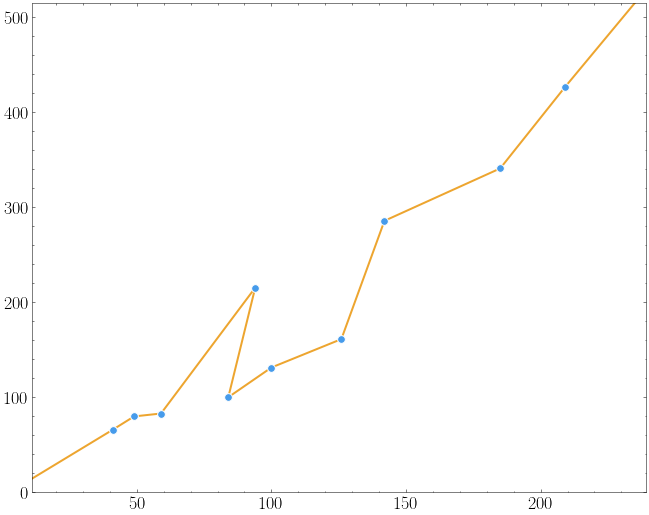
\includegraphics[width=12cm]{images/state-of-art/overfitting/overfitting.png}
    \caption{Ejemplo de \textit{overfitting} en una regresión lineal.}
    \label{fig:basic_network}
\end{figure}

manteniendo la precisión de los datos de prueba mientras nuestra red se entrena. 

Una de las maneras más rápidas de saber si un modelo se está entrenando con \textit{overfitting} es usando un segundo dataset además del de entrenamiento. Normalmente, antes de crear una red neuronal hay que realizar un preprocesado de datos explicadas en la Sección TODO. Como bien se explica en esa sección, el dataset original se suele dividir en tres dataset distintos: entrenamiento, validación y test. Obviamente, el \textit{dataset} de entrenamiento es usado para entrenar e ir ajustando los parámetros de las matrices $W$ de forma iterativa. Por otro lado, se tiene los \textit{datasets} de validación y test que son usados para evaluar distintas métricas. Si el problema que se quiere resolver con la red es de tipo regresión se suele usar como métrica algún tipo de error explicados en la Sección \ref{costfunction} como por ejemplo: \textit{MAE}, \textit{MSE} o error de \textit{Huber}. Por otro lado si el problema a resolver es de clasificación, se suele usar la precisión como métrica.
\newline

Si vemos que la precisión de los datos de prueba ya no mejora, entonces deberíamos dejar de entrenar. Por supuesto, en sentido estricto, esto no es necesariamente un signo de \textit{overfitting}. Podría ser que la precisión de los datos de la prueba y los datos de entrenamiento dejen de mejorar al mismo tiempo. Aún así, la adopción de esta estrategia evitará el exceso de adaptación.
\newline

Al finalizar de cada \textit{epoch}, se usarán un subconjunto de datos del \textit{dataset} de entrenamiento y otro subconjunto del \textit{dataset} de validación. Con ellos, se calculará el valor de la métrica seleccionada y se obtendran dos valores. Estos valores se puede comparar entre ellos. Dos valores que son parecidos indican que el modelo es capaz de estrapolar a otros casos que no ha usado para el entramiento. Por el contrario, si el valor asociado al \textit{dataset} de entrenamiento es mucho mejor que el asociado al de validación esto puede significar que el modelo pueda estar sufriendo de \textit{overfitting}. Un entrenamiento llevado a cabo sin \textit{overfitting} se puede visualizar en la figura TODO.
\newline

Al inicio del entrenamiento, como la red no ha sido entrenada y los paramétros inicializados aleatoriamente, el modelo tendrá unas métricas bastantes malos, es decir, si se está usando algún error, dicho valor será muy alto. Por otro lado si se está midiendo la precisión del modelo dicho valor distará mucho del 100\%. Estas métricas serán igualmente malas tanto para ambos \textit{datasets}. Según vayan ocurriendo \textit{epochs} en el entrenamiento, llegará un momento que el modelo no pueda mejorar más y comenzará a memorizar los datos con los que esta siendo entrenado del \textit{dataset} de entrenamiento provocando que la métrica asociada al entrenamiento sea casi perfecta y la de validación progresivamente vaya empeorando. Un ejemplo de un entremiento que sufre de \textit{overfitting} puede verse de la siguiente manera:
\newline

\begin{figure}[H]
    \centering
    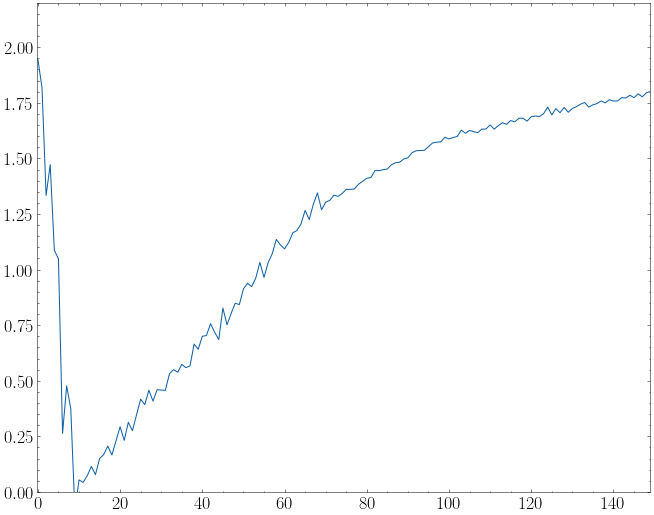
\includegraphics[width=12cm]{images/state-of-art/overfitting/overfitting-loss.png}
    \caption{Ejemplo de \textit{overfitting} en una regresión lineal usando un error como métrica.}
    \label{fig:basic_network}
\end{figure}

Al comienzo del entrenamiento ambas métricas van en pararelo, hasta que llegan a la \textit{epoch} X, en ese punto se puede visualizar como la métrica de validación poco a poco va empeorando. Es en ese punto donde se ve que la red tiene un problema de \textit{overfitting}. Dependiendo de la métrica usada, el \textit{overfitting} puede aparecer antes o después, pero es un tema más complejo que no se explicará en este trabajo.
\newline

Aún así hay varias técnicas que se explicarán a continuación para evitar el \textit{overfitting}: 
\begin{itemize}
    \item Regularización L1 y L2:
    Son dos métodos que calculan un valor conocido como penalización que se añade al error y de ese modo poder penalizar parámetros con valores grandes. Si una neurona tiene valores grandes puede ser signo de que la neurona está intentando memorizar. De hecho, se considera una mala práctica dejar que un conjunto pequeño de neuronas de la red sean las que más responsabilidad tengan, es decir, que sus parámetros asociados sean muy grandes.
    \newline
    
    Por un lado, se tiene L1 que es la suma de todos los valores absolutos de $w$ y $b$. Es una penalización linear ya que la función asociada es directamente proporcional a los parámetros. La penalización L2 es la suma de todos los parámetros $w$ y $b$ al cuadrado. Es una función no lineal y penaliza con mayor intensidad a os valores grande a diferencia de L1 que penaliza mucho más en proporción a los valores pequeños por ser lineal. Esto causa que el modelo empieza a ser invariante a pequeños valores de entrada y variante solo a los valores grandes. Por ello, L1 es raramente usado a nor ser que sea en combinación con L2. Ambas funciones están en función de un valor $\lambda$, con este valor se puede dictar cuanto impacto tendrá L1 y L2 en el error final. Matemáticamente:
    
    \begin{align*}
         L_{1w} = \lambda \sum_m |w_m| &&  L_{2w} = \lambda \sum_m w^2_m \addtocounter{equation}{1}\tag{\theequation} \\ 
         L_{1b} =\lambda \sum_n |b_n| && L_{2b} = \lambda \sum_n b^2_n \addtocounter{equation}{1}\tag{\theequation}
    \end{align*}
    

    El error final viene dado por la simple suma del error calculado por la función de coste y L1 con L2:
    \begin{equation}
        c_T = c + L_{1w} + L_{1b} + L_{2w} + L_{2b}
    \end{equation}
    
    Como se usa la regularización para el calculo de $c$, hace falta saber su derivada para poder usar el \textit{back-propagation}. Quedando la derivada de coste de la siguiente forma:
    
    \begin{equation}
        \frac{\partial c_T}{\partial w^{L_i}} = c' + L'_{1w} + L'_{1b} + L'_{2w} + L'_{2b}
    \end{equation}
    
    Las derivadas de L1 y L2 son las siguientes:
    \begin{align*}
         L'_{1w} = \lambda \begin{cases} 1,& \text{si } w_m > 1\\ -1,& \text{si } w_m < 1\end{cases} && L'_{2w} =  2\lambda w_m \addtocounter{equation}{1}\tag{\theequation} \\ 
         L'_{1b} =  \lambda \begin{cases} 1,& \text{si } b_n > 1\\ -1,& \text{si } b_n < 1\end{cases} && L'_{2b} = 2\lambda b_n \addtocounter{equation}{1}\tag{\theequation}
    \end{align*}
    
    \item \textit{Dropout} \label{dropout}: Usando esta técnica, en cada iteración del entrenamiento la red se modifica. Supongamos que se tiene un \textit{input} $x$ y el valor deseado $y$. Ordinariamente, se entrenaría mediante la propagación hacia adelante de $x$ a través de la red, y luego la propagación hacia atrás para determinar la contribución al gradiente. Con \textit{dropout}, este proceso se modifica. Se comienza eliminando aleatoriamente (y temporalmente) un porcentaje de las neuronas ocultas en la red, mientras que se deja las neuronas de entrada y salida sin modificar. Las neuronas que han sido borradas, serán neuronas "fantasmas" para ese \textit{epoch}:
    
    \begin{figure}[H]
        \centering
        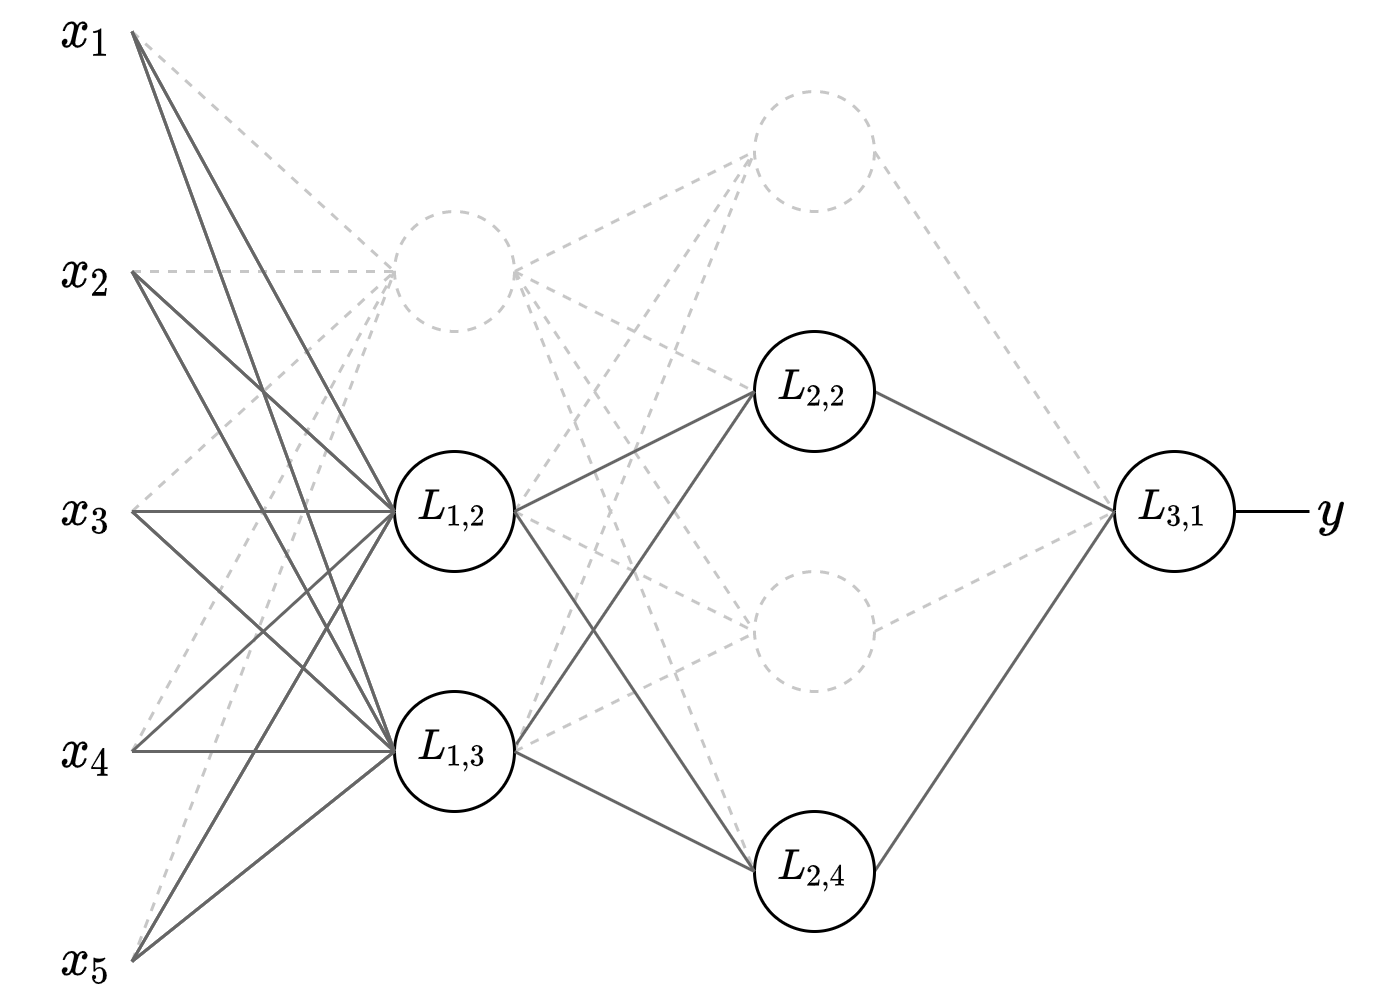
\includegraphics[width=12cm]{images/state-of-art/overfitting/dropout-1.png}
        \caption{\textit{Dropout} aplicado a una red con un $50\%$  de probabilidades}
        \label{fig:basic_network}
    \end{figure}
    
    Una vez terminado el proceso de propagación hacia adelante y \textit{backpropagation}, se comenzará un nuevo \textit{epoch} eliminando aleatoriamente un conjunto de neuronas. Es resumen, por cada iteración, se eliminar un subconjunto de las neuronas de acuerdo a un porcentaje dado.
    \newline
    
    Repitiendo este proceso durante toda la fase de entrenamiento, la red aprenderá unas matrices $W$ que se habrán aprendido en condiciones en las que un subconjunto de las neuronas ocultas fueron eliminadas. Cuando realmente se ejecuta la red completa, significará que el número de neuronas activas será mayor. Por ello, se compensar reduciendo la parte proporcional con las que fueron entradas. Por ejemplo, usando un porcentaje igual a $50$, los valores de $W$ serán la mitad de lo que el gradiente haya calculado.
    

\end{itemize}

% Curse of dimensionalrity
%TODO Ejemplo de modelo normal vs modelo con overffiting

% L1 and L2 regularization

